\section{Literature Review} % (fold)
\label{sec:literature_review}

% section literature_review (end)

This section cover the literature review, as well as required background information on Bluetooth and ECG.

\subsection{Electrocardiogram} % (fold)
\label{sub:electrocardiogram}

Most of the reviewed WBAN literature discuss or mention ECG in some form or another, because of it's high technical requirements. However, we found many inconsistencies and simplifications about ECG, that in worst case may have invalidated parts of previously conducted research. Because of this, we spent some time understanding both the measurement itself and how it is carried . In the following section we introduce ECG before reviewing other research involving the diagnostic tool.

Electrocardiogram is a measurement of the electrical activity around the heart. The measurements are done by a set of external electrodes attached to the skin at certain places around the chest. These electrodes measure the depolarization of electrical charges that happen in the cell membranes covering the heart at every heart beat. An ECG is conducted by having either 3, 5 or 12 leads. The term lead refers to the voltage difference \textit{between a given pair} of electrodes, parallel to the direction of the lead. Based on the signal strength of each lead, cardiologists can get information about angles and properties of the heart. The leads can either be actual or derived from a vector model\footnote{ The Cabrera circle uses a vector representation to give a good overview of the different leads, and their relationship} based on 2 or more actual leads. Typically 5 electrodes can be used for a 3 and 5-lead ECG. It is however important to note that the amount of electrodes don't necessary correspond to the number of leads, and the amount of derived leads does not necessary correspond the the number of actual leads. The terminology here seem to confuse a lot of people, as we have seen and heard in both literature and in practice. Alesanco and García are among the few that describe this correctly in \cite{Alesanco:2010kc}, where they state that \textit{``(...) only eight leads should be transmitted since the other four can be derived from them''}. The this confusion is not unfounded, as there exist several techniques for deriving different leads from other leads. As we'll see later, a 12-lead EASI ECG may be derived from 5 electrodes capturing only 3 actual leads (or vectors). Even the traditional 12-lead ECG, is derived from 10 electrodes\footnote{ One at each extremity (limb) and 6 on the chest.} which capture 9 actual leads. The differences roles these leads play in practice, are discussed further in Section~\ref{sec:clinical_context}. The consequence of this confusion is that previous research either make incorrect assumptions or report ambiguous results that are hard to verify. Some research \cite{yubin:2012tr, Lee:2009bu, Alesanco:2010kc}, only consider 1 or 2 leads, which has been proven insufficient by~\cite{Drew:1998wp}.

\begin{figure}[H]
\centering
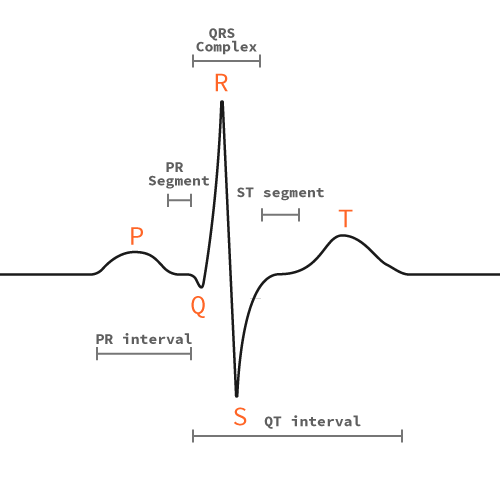
\includegraphics[scale=0.35]{img/figures/QRS.png}
\caption{QRS Complex with interval annotations}
\label{fig:qrsAnnotations}
\end{figure}

\noindent
After the leads are sampled in a wireless ECG solution, they can be streamed in raw, or compressed and optimized for transmission\cite{Balouchestani:2013dr, Alesanco:2010kc}. In order to reduce the scope of this project, we will only focus on the the core aspects of ECG. Different compression and low sampling techniques are therefore omitted completely. After being transmitted, the signals are analyzed at a processing unit, where common angles and intervals in the QRS complex as well as heart rate are calculated. The QRS complex as seen in Figure~\ref{qrsAnnotations} denotes the plot or graphical representation of the electrical signals. On a per lead basis, these plots are printed on gridded paper or displayed on a monitor. Cardiologists learn to analyze the leads and are able to make a diagnosis based on different intervals in the complex, among other things. An overview of some common intervals and the different cardiac diseases they indicate are presented in Table~\ref{tab:characteristicECGintervals}. Based on this analysis, the ECG system may automatically trigger alarms if certain thresholds in the intervals are exceeded.

\begin{table}[]
\centering
\caption{Characteristic ECG intervals from \cite{Jara:2012fi}}
\label{tab:characteristicECGintervals}
\begin{tabular}{|l|l|}
\hline
\textbf{Interval QRS \textgreater 120ms} & \begin{tabular}[c]{@{}l@{}}Ventricular hypertrophy, necrosis, BCRRD,\\ BCRI, pacemakers, cardiomyopathies,  \\ electrolyte abnormalities.\end{tabular}     \\ \hline
\textbf{Interval PQ \textgreater 200ms}  & Frist-degree AV block                                                                                                                                      \\ \hline
\textbf{Interval PR \textless 120ms}     & \begin{tabular}[c]{@{}l@{}}Tachycardia, WPW, manners or \\ headphones low rates.\end{tabular}                                                              \\ \hline
\textbf{Interval QT \textgreater 450ms}  & \begin{tabular}[c]{@{}l@{}}Antiarrhytmic medicines, ischemic heart deisease, \\ cardiomyopathies, hypocalcemia, mixedema, \\ long QT syndrome\end{tabular} \\ \hline
\textbf{Interval QT \textless 350ms}     & \begin{tabular}[c]{@{}l@{}}Hypercalcemia, hyperkalemia,  early \\ repolarization, digoxin\end{tabular}                                                     \\ \hline
\end{tabular}
\end{table}


We have reviewed several earlier projects involving wireless ECG. Some of them are mentioned here, while others will be discussed in Section~\ref{sub:wireless_body_area_networks} and~\ref{sub:bluetooth}.

% subsection electrocardiogram (end)

\subsection{Wireless Body Area Networks} % (fold)
\label{sub:wireless_body_area_networks}

% The notion of a mobile gateway has been widely adopted and discussed \cite{Movassaghi:2014hi, Mohammed:2014dw, Touati:2015gy, EmilJovanov:2005ty} in earlier research.
Missing.
% TODO mention the differnt classes of prioritized data

% subsection wireless_body_area_networks (end)

\subsection{Bluetooth and ambulatory ECG} % (fold)
\label{sub:bluetooth}

As we'll see in later sections, Bluetooth was an attractive technology for us because of its widespread presence, as well as the low energy features introduced with version 4.0 of the specification. In this section we will cover the basics of Bluetooth Smart and discuss related research projects using the technology.

% Bluetooth was originally developed at Ericsson in (...). 

% (...) Because of confusion around the ``low energy'' devices and regular Bluetooth devices Bluetooth SIG announced their new branding strategy in 2011, with a new logo and name: Bluetooth Smart. Throughout this thesis we will use both the old Low Energy suffix as well as Bluetooth Smart (we should probably fix this?).

% GATT and Profiles
% The profile defines the types of state data that a device exposes and how that data can be used. Profiles are organized like this:
% Services > Characteristics and Descriptors.

% How are Bluetooth Smart profiles implemented? Efforts are being made by Bluetooth SIG to standardize data profiles in order to ensure interoperability between devices supporting the protocol. A profile for a type of device defines the GATT Services which a device of this type must or may implement. This is related to interoperability which we will cover in the next section.

% subsection bluetooth (end)

\subsection{Interoperability} % (fold)
\label{sub:interoperability}

Rahmani et. al. gives a clear overview of different forms of interoperability in their 2015 paper about Smart e-Health Gateways~\cite{DrAmirMohammadRahmani:2014vx}. They separate the concern of interoperability and reconfigurability into the following categories: Device interoperability, protocol interoperability, data interoperability, reconfigurability and device discovery and mobility support. In the following sections we will give an overview of data interoperability related to Bluetooth.

\subsubsection{Data Interoperability} % (fold)
\label{ssub:data_interoperability}

% subsubsection data_interoperability (end)

Document and message standardization in health care is a huge topic and certain actors like HL7 have been working actively with standardization development for the least 30 years. In this section we will cover WBAN related papers discussing interoperability as well as giving an brief overview of the latest standardization efforts made by actors like HL7, Continua and the Bluetooth SIG.

The Continua Alliance develops interoperability guidelines and offer device manufacturers a way of certifying their Bluetooth Smart devices for Personal Connected Health. Their guidelines are globally recognized as the only standard for Personal Connected Health \cite{newRef:27}. The certification program is organized as follows: Continua selects and approves certain GATT Profiles (aka. Smart Profiles). Devices that support these profiles can be certified, meaning that they will be compliant and that the data they deliver can be ``mapped into the Continua & HL7 Record-set and shared, where it can become available as needed to social media, care providers, hospitals, clinicians, etc.'' \cite{newRef:27}.

The GATT profiles are specified by the Bluetooth SIG through Device Data Specifications. This work is organized in different domains and there is a specific sub-group for Health Device Profiles (HDP) (current version 1.1), some of whom are approved by Continua. HDP defines devices as either sinks and/or sources. In this thesis these roles are referred to as as nodes and personal mobile gateways.

The HDP specification does not specify the format nor content transmitted, but confine to ISO/IEEE 11073-20601 Personal Health Data Exchange Protocol \cite{newRef:18} Bluetooth SIG require devices implementing the HDP to follow the ISO standard for exchanging data between HDP devices and IEE 11073-104xx Device Specification. form ISO/IEEE 11073-20601 Data Exchange Specification. ISO/IEEE draws a clear line between consumer electronics and medical devices: 

``Provides strong application level interoperability by operating with the ISO/IEEE 11073-20601 Personal Health Data Exchange Protocol [7], which defines a transport-agnostic Data Exchange Protocol and representation of device application data based on international standards.''

% ``This standard defines a common core of communication functionality for personal telehealth basic ECG (1- to 3-lead ECG) devices. Monitoring ECG devices are distinguished from diagnostic ECG equipment with respect to including support for wearable ECG devices, limiting the number of leads supported by the equipment to three, and not requiring the capability of annotating or analyzing the detected electrical activity to determine known cardiac phenomena. This standard is consistent with the base framework and allows multifunction implementations by following multiple device specializations (e.g., ECG and respiration rate).'' \cite{newRef:18}

% The Health Device Profile specification mention ECG as an example of data transmitted on Streaming Data Channels,


% subsection interoperability (end)

% section section_name (end)